\documentclass[a4paper,landscape,9pt]{article}

\usepackage[margin=1cm]{geometry}
\usepackage{fontspec}
\setmainfont{TeX Gyre Pagella}
\usepackage{unicode-math}
\setmathfont{TeX Gyre Pagella Math}

\usepackage{tikz}
\usetikzlibrary{arrows.meta,calc,positioning,shapes.geometric}
\usepackage{microtype}

\pagestyle{empty}
\setlength{\parindent}{0pt}
\setlength{\parskip}{0.25em}

\tikzset{
  node-d/.style={draw,fill=black,regular polygon,regular polygon sides=6,minimum size=7mm,inner sep=0pt,text=white,font=\tiny\bfseries},
  node-a/.style={draw,fill=black!70,regular polygon,regular polygon sides=3,minimum size=7mm,inner sep=0pt,text=white,font=\tiny\bfseries},
  node-t/.style={draw,circle,minimum size=7mm,inner sep=0pt,line width=0.4pt,font=\tiny},
  node-o/.style={draw,fill=black!15,rectangle,minimum size=7mm,inner sep=0pt,font=\tiny},
  node-i/.style={draw,diamond,minimum size=8mm,inner sep=0pt,line width=0.4pt,font=\tiny},
  impl/.style={-{Latex[length=1.2mm]},line width=0.3pt,black!80},
  exemp/.style={-{Latex[length=1.2mm]},line width=0.3pt,dashed,black!80},
  post/.style={-{Latex[length=1.2mm]},line width=0.3pt,dotted,black!80},
  band/.style={font=\scriptsize\scshape,text=black!60},
  bandline/.style={draw,black!18,line width=0.3pt},
}

\begin{document}

\begin{center}
{\large\scshape Proposisjonsgraf, seksjon 2}\hspace{0.8em}{\itshape Ikkje alle posisjonar er like sannsynlege}
\end{center}

\vspace{-0.6em}

\begin{center}
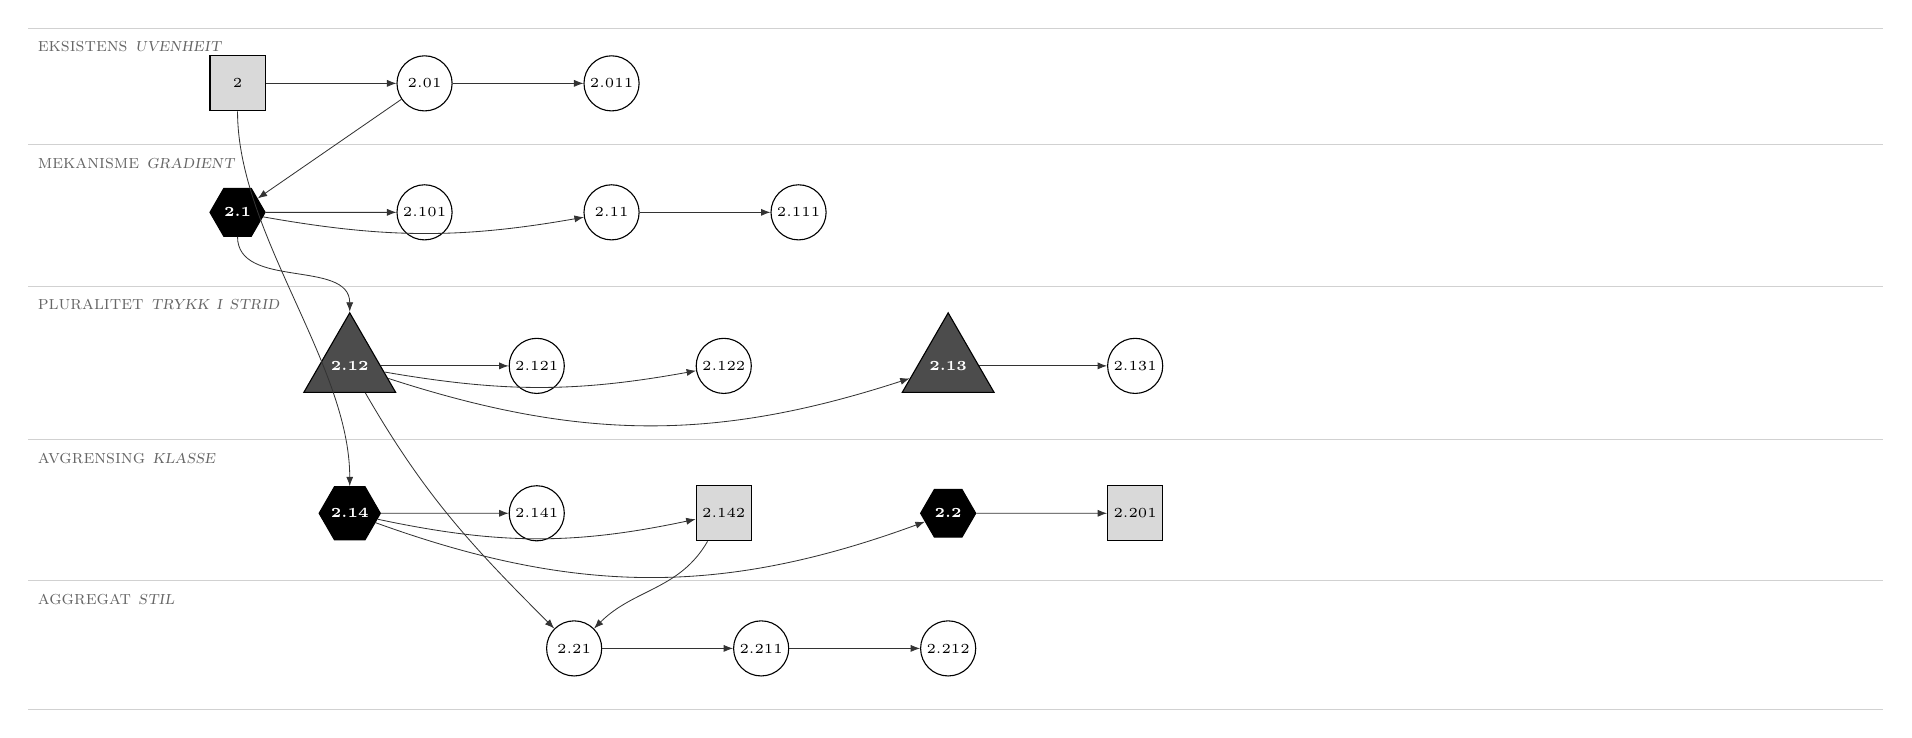
\begin{tikzpicture}[x=0.95cm,y=0.78cm]

  \draw[bandline] (-0.3, 0.6)   -- (24.5, 0.6);
  \draw[bandline] (-0.3, -1.3)  -- (24.5, -1.3);
  \draw[bandline] (-0.3, -3.6)  -- (24.5, -3.6);
  \draw[bandline] (-0.3, -6.1)  -- (24.5, -6.1);
  \draw[bandline] (-0.3, -8.4)  -- (24.5, -8.4);
  \draw[bandline] (-0.3, -10.5) -- (24.5, -10.5);

  \node[band,anchor=west] at (-0.3, 0.3)  {eksistens  \itshape uvenheit};
  \node[band,anchor=west] at (-0.3, -1.6) {mekanisme  \itshape gradient};
  \node[band,anchor=west] at (-0.3, -3.9) {pluralitet  \itshape trykk i strid};
  \node[band,anchor=west] at (-0.3, -6.4) {avgrensing  \itshape klasse};
  \node[band,anchor=west] at (-0.3, -8.7) {aggregat  \itshape stil};

  % BAND 1: eksistens
  \node[node-o] (p2)     at (2.5, -0.3)  {2};
  \node[node-t] (p201)   at (5, -0.3)    {2.01};
  \node[node-t] (p2011)  at (7.5, -0.3)  {2.011};
  \draw[impl] (p2)   -- (p201);
  \draw[impl] (p201) -- (p2011);

  % BAND 2: mekanisme
  \node[node-d] (p21m)   at (2.5, -2.4)  {2.1};
  \node[node-t] (p2101)  at (5, -2.4)    {2.101};
  \node[node-t] (p211m)  at (7.5, -2.4)  {2.11};
  \node[node-t] (p2111)  at (10, -2.4)   {2.111};
  \draw[impl] (p201)  -- (p21m);
  \draw[impl] (p21m)  -- (p2101);
  \draw[impl] (p21m)  to[bend right=10] (p211m);
  \draw[impl] (p211m) -- (p2111);

  % BAND 3: pluralitet (postulater!)
  \node[node-a] (p212)   at (4, -4.9)    {2.12};
  \node[node-t] (p2121)  at (6.5, -4.9)  {2.121};
  \node[node-t] (p2122)  at (9, -4.9)    {2.122};
  \node[node-a] (p213)   at (12, -4.9)   {2.13};
  \node[node-t] (p2131)  at (14.5, -4.9) {2.131};
  \draw[impl] (p21m)  to[out=-90,in=90] (p212);
  \draw[impl] (p212)  -- (p2121);
  \draw[impl] (p212)  to[bend right=10] (p2122);
  \draw[impl] (p212)  to[bend right=18] (p213);
  \draw[impl] (p213)  -- (p2131);

  % BAND 4: avgrensing (klasse og affordanse)
  \node[node-d] (p214d)  at (4, -7.3)    {2.14};
  \node[node-t] (p2141)  at (6.5, -7.3)  {2.141};
  \node[node-o] (p2142)  at (9, -7.3)    {2.142};
  \node[node-d] (p22d)   at (12, -7.3)   {2.2};
  \node[node-o] (p2201)  at (14.5, -7.3) {2.201};
  \draw[impl] (p2)     to[out=-90,in=90,looseness=0.8] (p214d);
  \draw[impl] (p214d)  -- (p2141);
  \draw[impl] (p214d)  to[bend right=12] (p2142);
  \draw[impl] (p214d)  to[bend right=20] (p22d);
  \draw[impl] (p22d)   -- (p2201);

  % BAND 5: aggregat (konfluens hjå 2.21)
  \node[node-t] (p221)   at (7, -9.5)    {2.21};
  \node[node-t] (p2211)  at (9.5, -9.5)  {2.211};
  \node[node-t] (p2212)  at (12, -9.5)   {2.212};
  \draw[impl] (p212)  to[out=-60,in=135] (p221);
  \draw[impl] (p2142) to[out=-120,in=45] (p221);
  \draw[impl] (p221)  -- (p2211);
  \draw[impl] (p2211) -- (p2212);

\end{tikzpicture}
\end{center}

\vspace{-0.2em}

\hrule

\vspace{0.4em}

\begin{minipage}[t]{0.325\textwidth}
{\scshape\small Lesing ovanfrå}

Rota \emph{2} seier at fordelinga over formrommet ikkje er einsarta. Band 1 trekk ut dei umiddelbare konsekvensane: noko verkar, og det som verkar er avgrensing, ikkje kraft (\emph{2.011}).

Band 2 definerer mekanismen som eit \textbf{seleksjonstrykk} (\emph{2.1}), ein gradient. Frå denne definisjonen veks fire teorem som spesifiserer kva trykket er og kva det ikkje er.

Seksjonens fyrste \emph{risiko} kjem i band 3. Her finn vi dei to postulata (triangla) som ber heile rammeverket: at fleire trykk verkar samstundes (\emph{2.12}), og at minst to peikar i motstridande retningar (\emph{2.13}).
\end{minipage}\hfill
\begin{minipage}[t]{0.325\textwidth}
{\scshape\small Lesing nedover}

Band 4 introduserer det som trykka opererer innanfor: \textbf{klassen}, avgrensa gjennom delt affordansestruktur (\emph{2.14}), og \textbf{materialaffordansen} som spesifikt lag (\emph{2.2}). Her kjem dei to fyrste empiriske observasjonane i traktaten, fylte kvadrat: \emph{2.142} om stil framfor materiale som prediktor, og \emph{2.201} om stål som låg klart i eit halvt hundreår før nokon såg stolen i røyret.

Band 5 er seksjonens konfluens. \emph{2.21} har to foreldre: postulatet om pluralitet (\emph{2.12}) og den empiriske observasjonen (\emph{2.142}). Saman genererer dei innsikta at \textbf{stilen} er eit aggregat, ikkje ei årsak. Dette er seksjonens heimkomst.
\end{minipage}\hfill
\begin{minipage}[t]{0.325\textwidth}
{\scshape\small Strukturelle innsikter}

\emph{Fyrste triangla.} Seksjonen inneheld seksjonen sine fyrste postulat. Det er her teorien byrjar å tru på noko.

\emph{Fyrste empiri.} \emph{2.142} og \emph{2.201} er dei fyrste fylte kvadrata i traktaten. Teorien møter stoffet sitt her.

\emph{Konfluens hjå} \emph{2.21.} Som \emph{1.22} i seksjon 1, har \emph{2.21} to foreldre. Det er ikkje tilfeldig at kvar seksjon ser ut til å slutte i eit syntesepunkt.

\emph{Asymmetri.} Sjølv om \emph{2.14} og \emph{2.2} greiner ut horisontalt, er det berre \emph{2.142} som sender ei pil nedover til band 5. \emph{2.201} heng som fri illustrasjon av \emph{2.2}; han bind ikkje noko vidare. Ikkje all empiri ber same vekt.
\end{minipage}

\end{document}
